\documentclass[tikz,border=5pt]{standalone}
\usepackage{tikz}
\usepackage{lmodern}
\usetikzlibrary{shapes,arrows,positioning,calc,fit}

\begin{document}
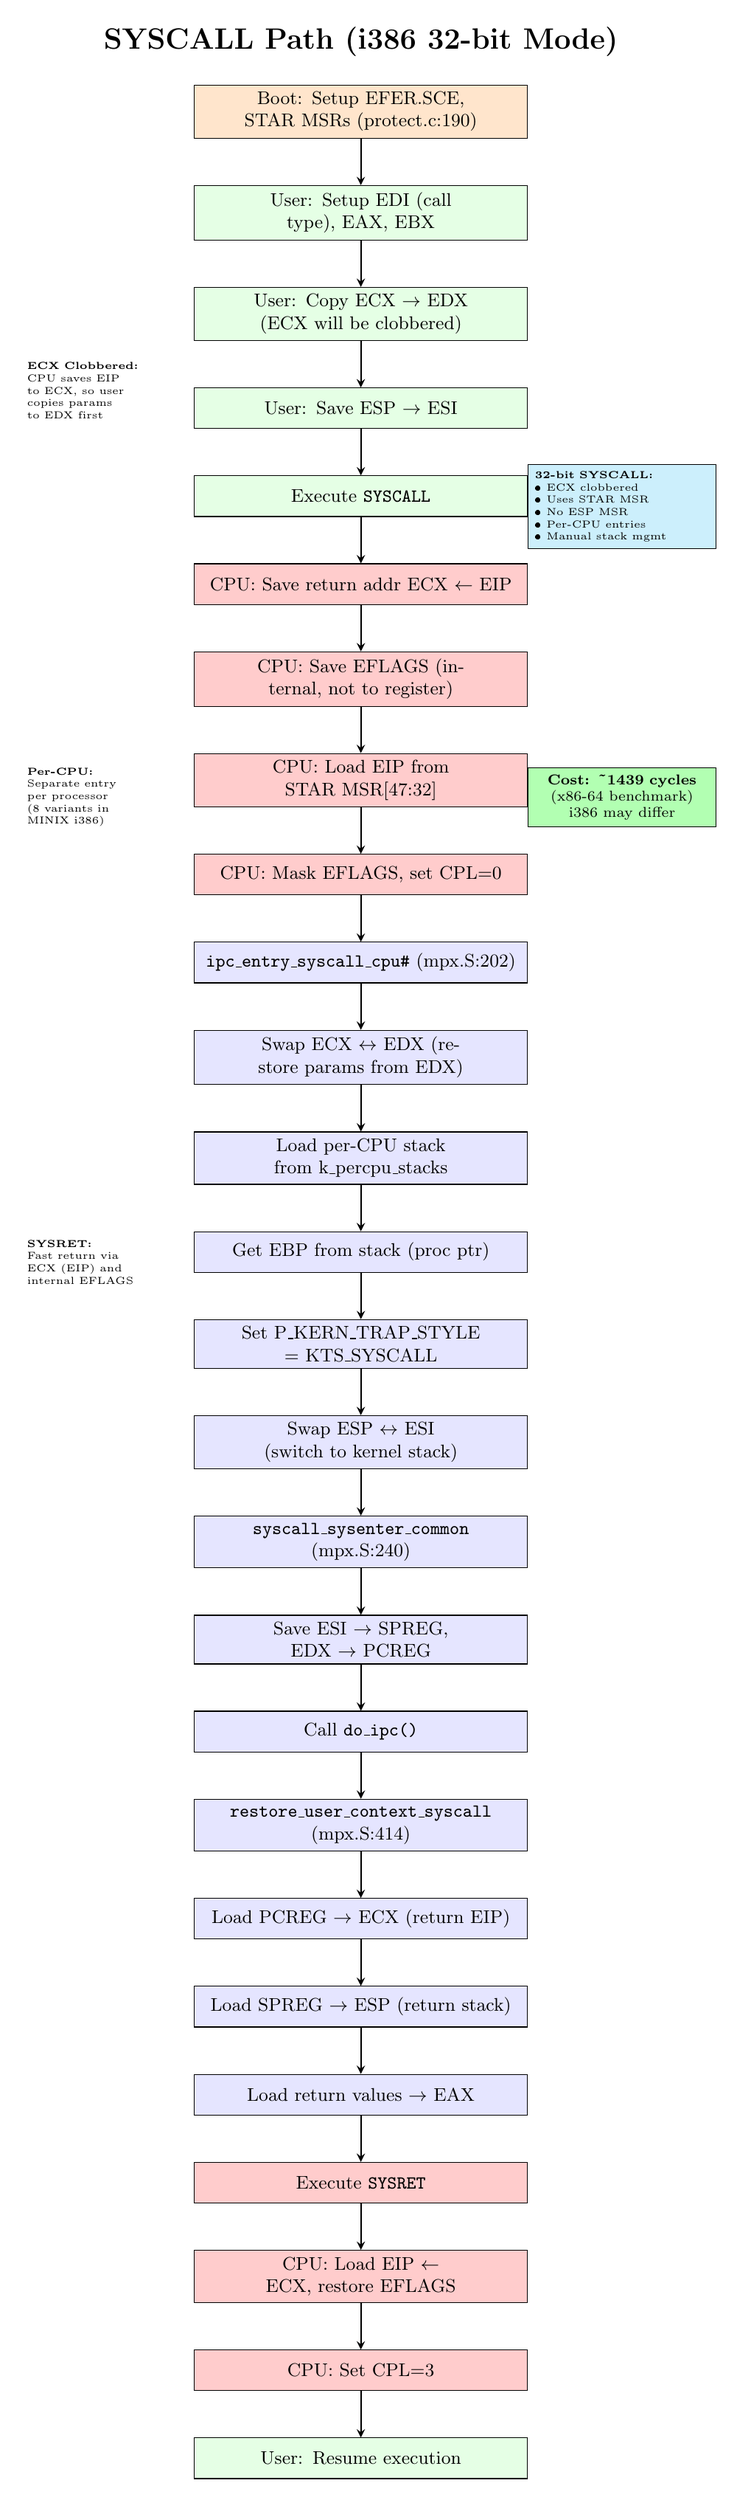
\begin{tikzpicture}[
    node distance=0.8cm,
    box/.style={rectangle, draw, fill=blue!10, text width=5.5cm, align=center, minimum height=0.7cm, font=\small},
    hw/.style={rectangle, draw, fill=red!20, text width=5.5cm, align=center, minimum height=0.7cm, font=\small},
    user/.style={rectangle, draw, fill=green!10, text width=5.5cm, align=center, minimum height=0.7cm, font=\small},
    arrow/.style={->,>=stealth,thick}
]

% Title
\node[font=\Large\bfseries] at (0,0) {SYSCALL Path (i386 32-bit Mode)};

% MSR Setup (boot time)
\node[box, fill=orange!20] (msr) at (0,-1.2) {Boot: Setup EFER.SCE, STAR MSRs (protect.c:190)};

% User space prep
\node[user] (user1) [below=of msr] {User: Setup EDI (call type), EAX, EBX};
\node[user] (user2) [below=of user1] {User: Copy ECX $\rightarrow$ EDX (ECX will be clobbered)};
\node[user] (user3) [below=of user2] {User: Save ESP $\rightarrow$ ESI};
\node[user] (user4) [below=of user3] {Execute \texttt{SYSCALL}};

% Hardware actions (32-bit mode)
\node[hw] (hw1) [below=of user4] {CPU: Save return addr ECX $\leftarrow$ EIP};
\node[hw] (hw2) [below=of hw1] {CPU: Save EFLAGS (internal, not to register)};
\node[hw] (hw3) [below=of hw2] {CPU: Load EIP from STAR MSR[47:32]};
\node[hw] (hw4) [below=of hw3] {CPU: Mask EFLAGS, set CPL=0};

% Kernel entry (per-CPU)
\node[box] (kern1) [below=of hw4] {\texttt{ipc\_entry\_syscall\_cpu\#} (mpx.S:202)};
\node[box] (kern2) [below=of kern1] {Swap ECX $\leftrightarrow$ EDX (restore params from EDX)};
\node[box] (kern3) [below=of kern2] {Load per-CPU stack from k\_percpu\_stacks};
\node[box] (kern4) [below=of kern3] {Get EBP from stack (proc ptr)};
\node[box] (kern5) [below=of kern4] {Set P\_KERN\_TRAP\_STYLE = KTS\_SYSCALL};
\node[box] (kern6) [below=of kern5] {Swap ESP $\leftrightarrow$ ESI (switch to kernel stack)};
\node[box] (kern7) [below=of kern6] {\texttt{syscall\_sysenter\_common} (mpx.S:240)};
\node[box] (kern8) [below=of kern7] {Save ESI $\rightarrow$ SPREG, EDX $\rightarrow$ PCREG};
\node[box] (kern9) [below=of kern8] {Call \texttt{do\_ipc()}};

% Return path
\node[box] (ret1) [below=of kern9] {\texttt{restore\_user\_context\_syscall} (mpx.S:414)};
\node[box] (ret2) [below=of ret1] {Load PCREG $\rightarrow$ ECX (return EIP)};
\node[box] (ret3) [below=of ret2] {Load SPREG $\rightarrow$ ESP (return stack)};
\node[box] (ret4) [below=of ret3] {Load return values $\rightarrow$ EAX};
\node[hw] (hw5) [below=of ret4] {Execute \texttt{SYSRET}};
\node[hw] (hw6) [below=of hw5] {CPU: Load EIP $\leftarrow$ ECX, restore EFLAGS};
\node[hw] (hw7) [below=of hw6] {CPU: Set CPL=3};
\node[user] (user5) [below=of hw7] {User: Resume execution};

% Arrows
\foreach \i/\j in {msr/user1, user1/user2, user2/user3, user3/user4, user4/hw1, hw1/hw2, hw2/hw3, hw3/hw4, hw4/kern1, kern1/kern2, kern2/kern3, kern3/kern4, kern4/kern5, kern5/kern6, kern6/kern7, kern7/kern8, kern8/kern9, kern9/ret1, ret1/ret2, ret2/ret3, ret3/ret4, ret4/hw5, hw5/hw6, hw6/hw7, hw7/user5} {
    \draw[arrow] (\i) -- (\j);
}

% Side annotations
\node[font=\tiny, text width=2.5cm, align=left] at (-4.5,-6) {
    \textbf{ECX Clobbered:}\\
    CPU saves EIP\\
    to ECX, so user\\
    copies params\\
    to EDX first
};

\node[font=\tiny, text width=2.5cm, align=left] at (-4.5,-13) {
    \textbf{Per-CPU:}\\
    Separate entry\\
    per processor\\
    (8 variants in\\
    MINIX i386)
};

\node[font=\tiny, text width=2.5cm, align=left] at (-4.5,-21) {
    \textbf{SYSRET:}\\
    Fast return via\\
    ECX (EIP) and\\
    internal EFLAGS
};

% Cycle cost annotation
\node[font=\scriptsize, fill=green!30, draw, text width=3cm, align=center] at (4.5,-13) {
    \textbf{Cost: \textasciitilde1439 cycles}\\
    (x86-64 benchmark)\\
    i386 may differ
};

% Key differences box
\node[font=\tiny, fill=cyan!20, draw, text width=3cm, align=left] at (4.5,-8) {
    \textbf{32-bit SYSCALL:}\\
    • ECX clobbered\\
    • Uses STAR MSR\\
    • No ESP MSR\\
    • Per-CPU entries\\
    • Manual stack mgmt
};

\end{tikzpicture}
\end{document}
